\documentclass[11pt,a4paper]{article}
\usepackage{graphicx} % For including images
\usepackage{tabularx} % For flexible table widths
\usepackage{lipsum}   % For generating dummy text, can be removed
\usepackage[margin=1in]{geometry} % Adjust page margins as needed
\usepackage[export]{adjustbox}
\usepackage{float}
\usepackage{longtable}
\begin{document}

\title{Hardware spring reverb}
\author{Honglin Cao}
\date{\today}
\maketitle

\section{backstory}

For our project, I firstly googled and find some photos of reverb tanks for the guitar amp. Most of their designs has the transducer (both source and receive) pushing and pulling on a rod, and the rod is connected to the spring vertically to create a transverse wave on the spring and isolates the pulling force from the spring from the transducer.

However, this feature will means the design of the spring reverb will be much harder, so I go with connecting the spring directly to the transducer, and let the transducer pushing and pulling directly on the spring create longitudinal wave into the spring. This design might have some change on the characteristics of the resulting spring reverb, and sadly I have no time and resource to build a transverse version of the reverb. And this could also be an interesting topic to look into.

For the source, I come across some very nice looking surface transducer, which is meant to transfer vibrations to large surfaces to create audible sounds, and they are just essentially conventional speakers with the paper cone replaced by a piece of metal. Which means the amplitude of them will be significantly smaller than purposely-designed transducer found in off-the-shelf reverb tank, hopefully this will not causing any big issue on the results.

For receiving side, for simplicity I decided to just go with conventional guitar piezo under-saddle pickup to save some time on designing and manufacturing, and I can use my exising guitar amp to get a clean sound from it rather than use some cheap amplifier board for a transducer.

As for the springs, I have no idea what kind of springs reverb tank usually uses, so I can only source some stainless steel pulling springs (so they have 2 loop on both end to hook onto something) from aliexpress and ems-store from Engineering 3 with various diameter and length, hopefully will find a suitable one.

\newpage
\section{Design and Build Flow}

\begin{longtable}{| p{.3\textwidth} | p{.7\textwidth} |} 
\hline
\textbf{Photo} & \textbf{Description} \\
\hline

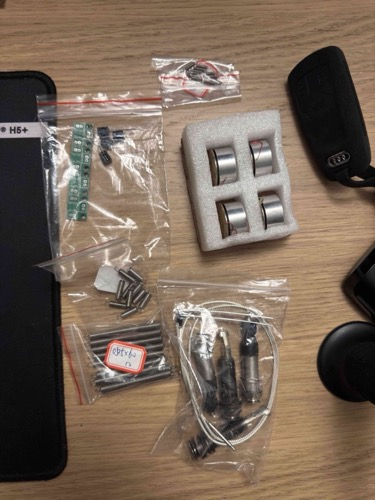
\includegraphics[width=0.3\textwidth,valign=c]{photos/IMG_7909.jpg} & 
purchased surface transducer, driver board for the transducer, guitar piezo pickup, 6.5mm audio jack and several metal springs. \\ 
\hline

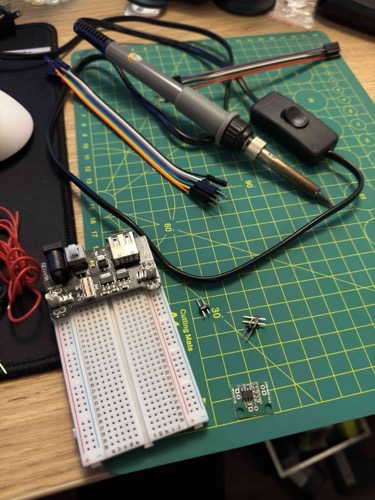
\includegraphics[width=0.3\textwidth,,valign=c]{photos/IMG_8080.jpg} & 
Used a power supply board and a bread board from my Arduino kit, prepare to solder the wires. \\ 
\hline

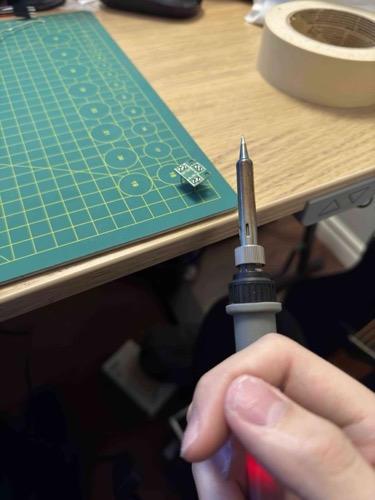
\includegraphics[width=0.3\textwidth,,valign=c]{photos/IMG_8082.jpg} & 
Soldered the pin to the transducer driver board. \\ 
\hline

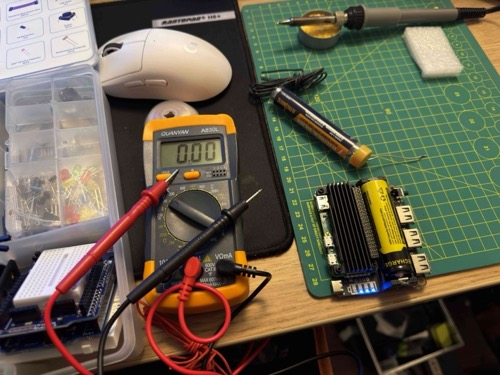
\includegraphics[width=0.3\textwidth,,valign=c]{photos/IMG_8084.jpg} & 
The power supply board needs 9V battery, trying to use my Raspberry PI Zero 2W to power the driver board instead. Used multimeter to determine the 5V and GND. \\ 
\hline

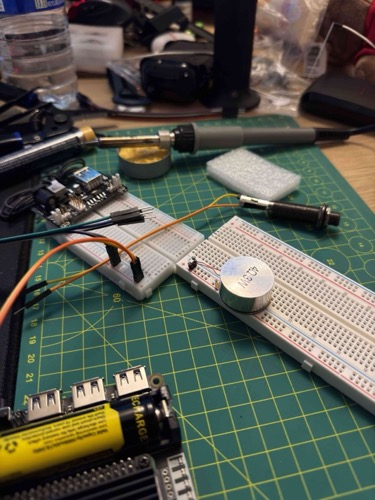
\includegraphics[width=0.3\textwidth,,valign=c]{photos/IMG_8085.jpg} & 
Soldered the surface transducer to a GPIO pin for easier connection later. \\ 
\hline

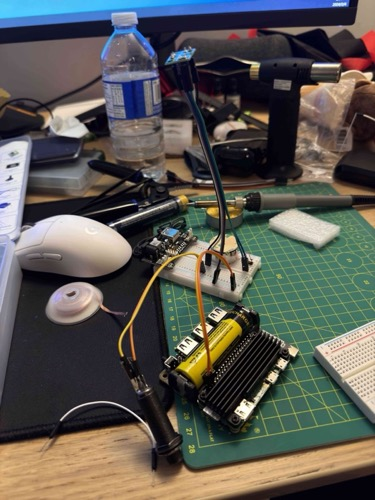
\includegraphics[width=0.3\textwidth,,valign=c]{photos/IMG_8086.jpg} & 
Connected both the driver board and the transducer itself to the bread board with Arduino cables. \\ 
\hline

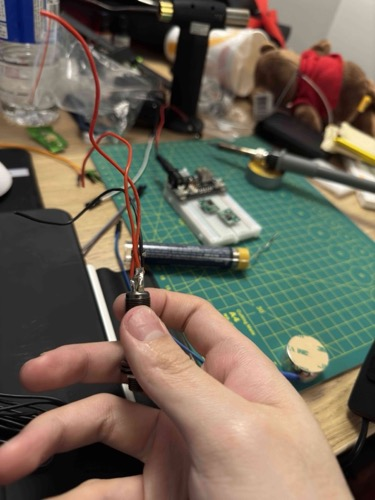
\includegraphics[width=0.3\textwidth,,valign=c]{photos/IMG_8095.jpg} & 
The 6.5 jack I purchased is stereo, even though we are only doing a mono output, but I soldered 3 wires to it. \\ 
\hline

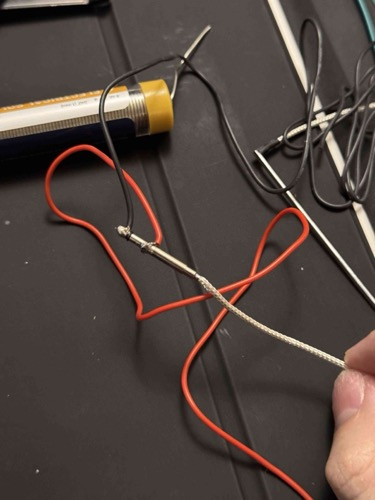
\includegraphics[width=0.3\textwidth,,valign=c]{photos/IMG_8096.jpg} & 
Soldered piezo pickup to 2 wires as well, i want to try to drive the piezo pickup with the transducer driver board. \\ 
\hline

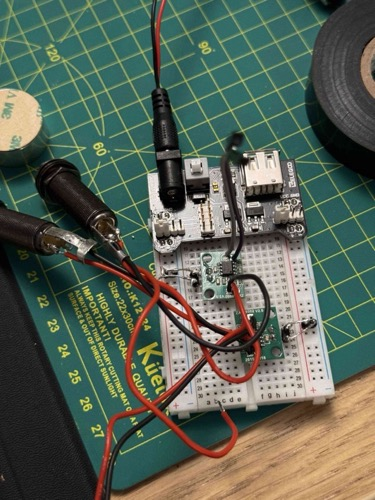
\includegraphics[width=0.3\textwidth,,valign=c]{photos/IMG_8097.jpg} & 
 Redo the GPIO pins only for 5V and GND so I can mount driver boards directly onto the bread board, and soldered the 6.5 Jack to the input and output of driver boards respectively, also soldered the piezo pickup to the input of one of the driver board.\\ 
\hline

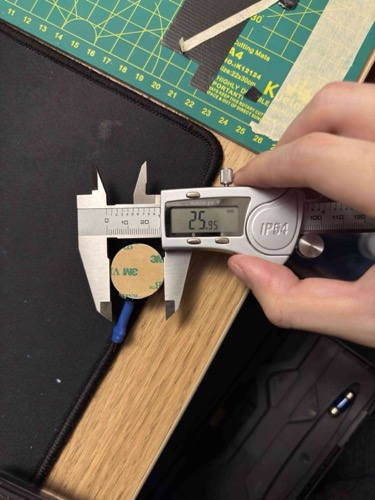
\includegraphics[width=0.09\textwidth,,valign=c]{photos/IMG_8745.jpg} 
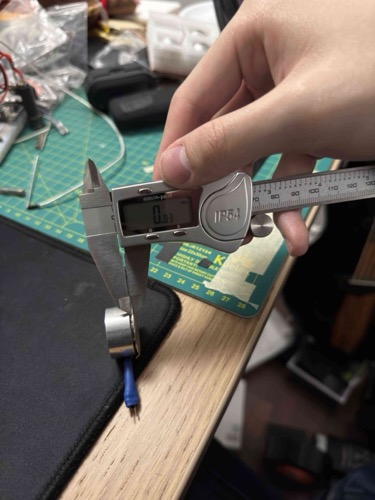
\includegraphics[width=0.09\textwidth,,valign=c]{photos/IMG_8746.jpg} 
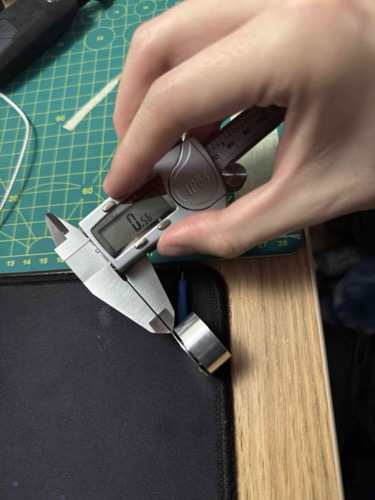
\includegraphics[width=0.09\textwidth,,valign=c]{photos/IMG_8748.jpg} & 
Measuring the dimension of the surface transducer for designing housing for the spring reverb. \\ 
\hline

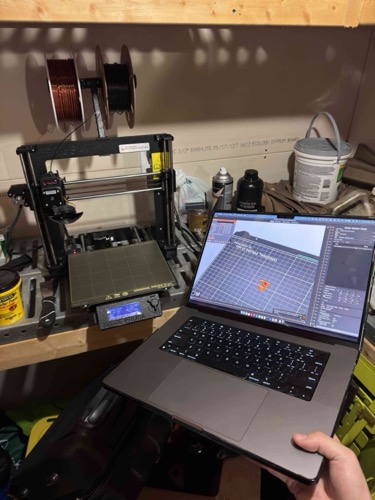
\includegraphics[width=0.3\textwidth,,valign=c]{photos/IMG_8749.jpg} & 
 Design and FDM 3D printed a hook that i will glue to the surface tranducer to hold the spring. \\ 
\hline

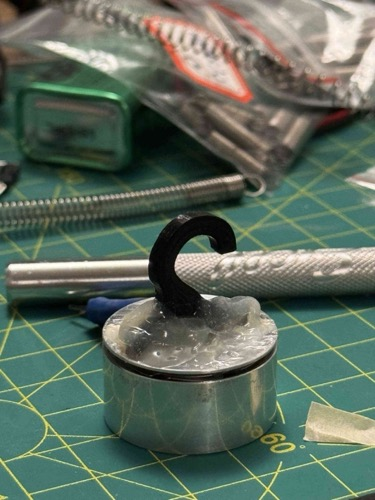
\includegraphics[width=0.3\textwidth,,valign=c]{photos/IMG_8767.jpg} & 
 Glued the hook to the surface transducer.\\ 
\hline

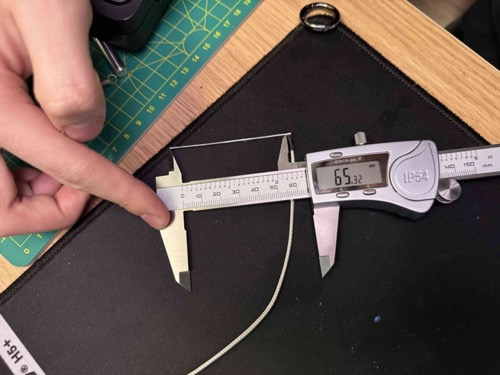
\includegraphics[width=0.09\textwidth,,valign=c]{photos/IMG_8770.jpg}
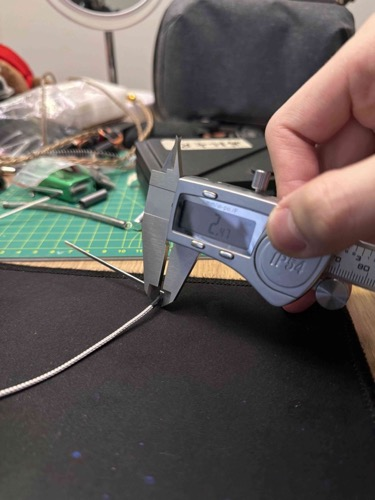
\includegraphics[width=0.09\textwidth,,valign=c]{photos/IMG_8771.jpg}
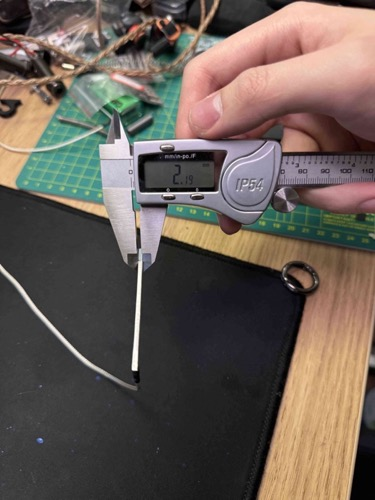
\includegraphics[width=0.09\textwidth,,valign=c]{photos/IMG_8772.jpg} & 
Doing some measurement on the piezo pickup for designing housing for spring reverb. \\ 
\hline

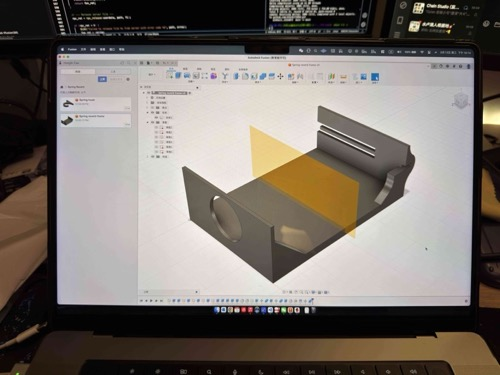
\includegraphics[width=0.14\textwidth,,valign=c]{photos/IMG_8773.jpg}
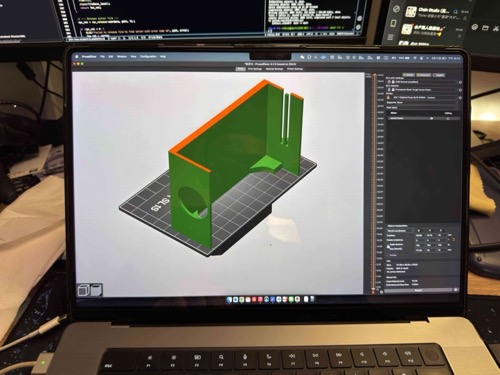
\includegraphics[width=0.14\textwidth,,valign=c]{photos/IMG_8774.jpg} & 
Designed the housing for spring reverb in Fusion 360, output to PrusSlicer for printing on SLA resin printer. \\ 
\hline

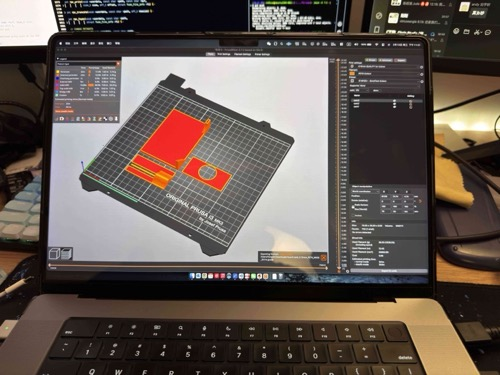
\includegraphics[width=0.3\textwidth,,valign=c]{photos/IMG_8776.jpg} & 
 Also designed a seperated version to glue on together later, just to make sure at least one version will be available.\\ 
\hline

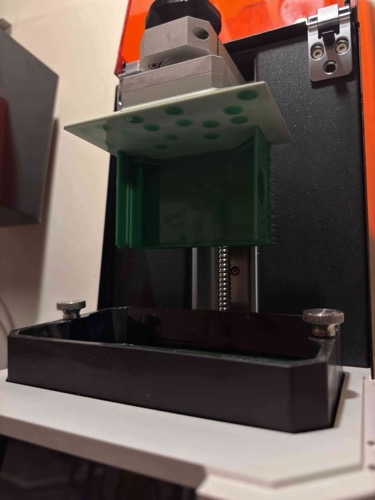
\includegraphics[width=0.3\textwidth,,valign=c]{photos/IMG_8779.jpg} & 
SLA resin print finished \\ 
\hline

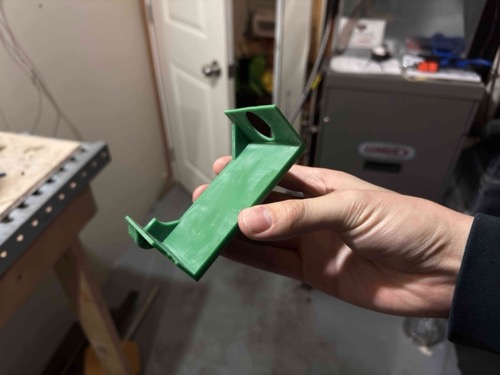
\includegraphics[width=0.3\textwidth,,valign=c]{photos/IMG_8783.jpg} & 
Post processing done \\ 
\hline

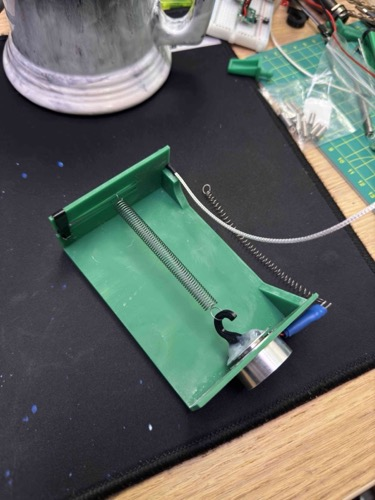
\includegraphics[width=0.3\textwidth,,valign=c]{photos/IMG_8784.jpg} & 
Mount components to the housing, dimension seems correct. \\ 
\hline

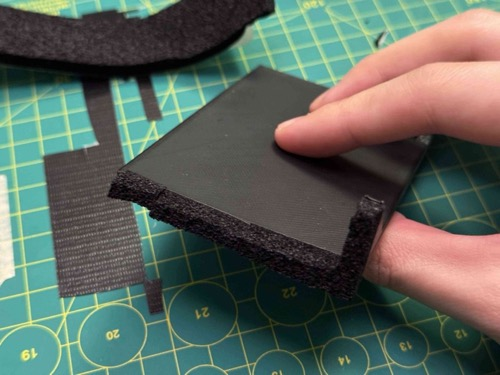
\includegraphics[width=0.3\textwidth,,valign=c]{photos/IMG_9382.jpg} & 
To prevent vibration of the surface transducer, applied automotive foam tape to the housing printed previously for gluing up. \\ 
\hline

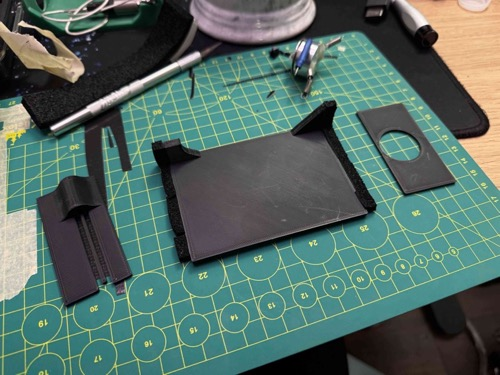
\includegraphics[width=0.3\textwidth,,valign=c]{photos/IMG_9383.jpg} & 
Applied foam tape to the two sides, so when bounding the 3 piece together the vibration wouldn't affect the piezo pickup system. \\ 
\hline

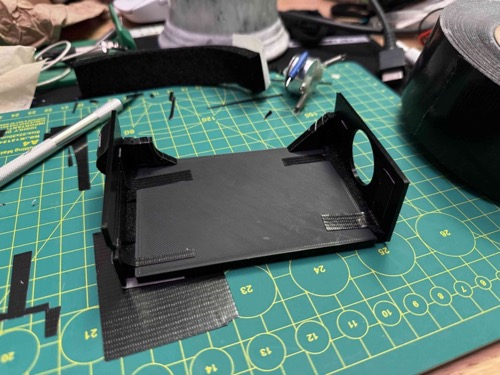
\includegraphics[width=0.3\textwidth,,valign=c]{photos/IMG_9384.jpg} & 
Connect the 3 piece using duct tape, so the joint (foam tape) is flexible and able to absorb vibrations.\\ 
\hline

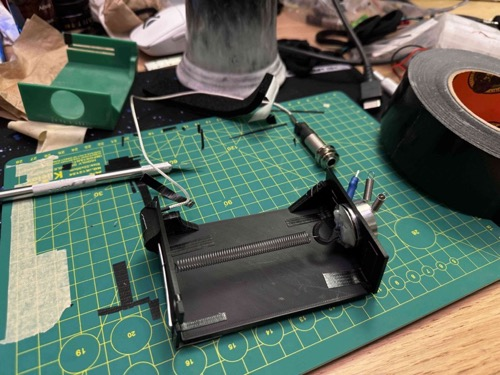
\includegraphics[width=0.3\textwidth,,valign=c]{photos/IMG_9385.jpg} & 
Installed all the components to the housing. \\ 
\hline

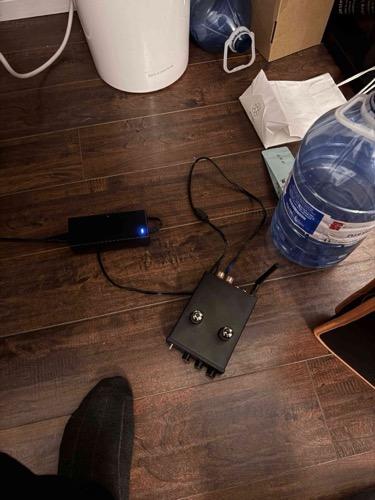
\includegraphics[width=0.3\textwidth,,valign=c]{photos/IMG_9593.jpg} & 
The amplifier for the surface transducer is broken somewhere, it's no longer functioning. Will use my bookshelf speaker amp to drive the surface transducer, it should be even better than the original amplifier I built for the surface transducer.\\ 
\hline

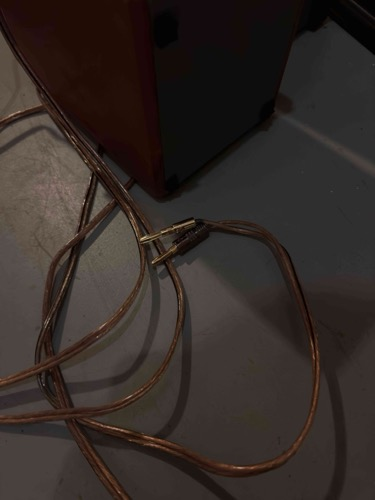
\includegraphics[width=0.3\textwidth,,valign=c]{photos/IMG_9594.jpg} & 
Take the speaker cable connector from my DIY bookshelf speaker \\ 
\hline

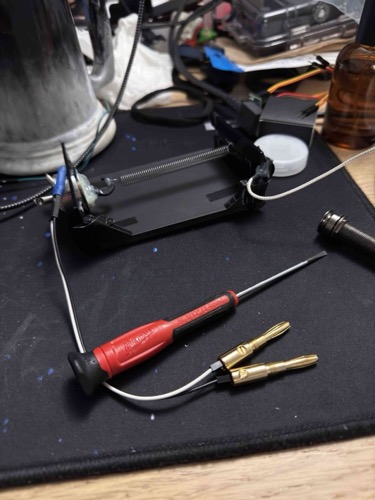
\includegraphics[width=0.3\textwidth,,valign=c]{photos/IMG_9596.jpg} & 
Connected the cable connector to the surface transducer. \\ 
\hline

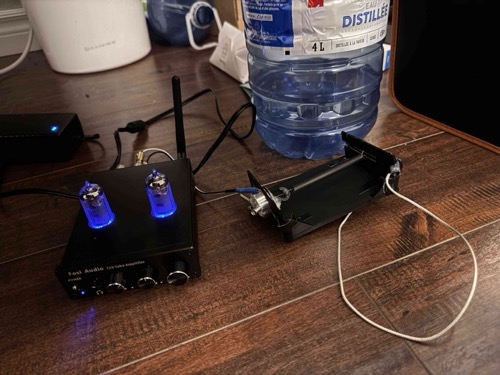
\includegraphics[width=0.3\textwidth,,valign=c]{photos/IMG_9597.jpg} & 
The amp works really well (it even has EQ adjustments), and the damping foam tape works as well, only around 20\% of the surface transducer's vibration is able to reach the plate housing the piezo pickup. Now it shouldn't affecting the piezo pickup anymore. \\ 
\hline

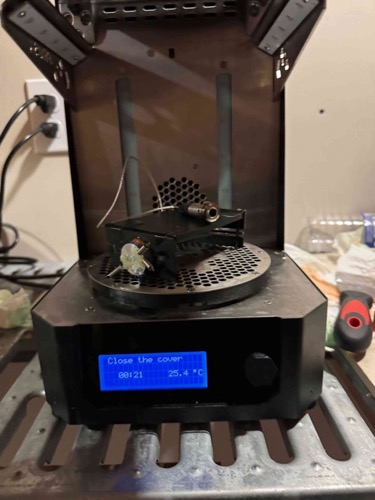
\includegraphics[width=0.3\textwidth,,valign=c]{photos/IMG_9603.jpg} & 
Some testing shows the surface transducer is moving inside the hole holding it creating some squeaking sound. Applied some UV curing resin to the surface transducer and using UV curing station for SLA printer to cure the resin. \\ 
\hline

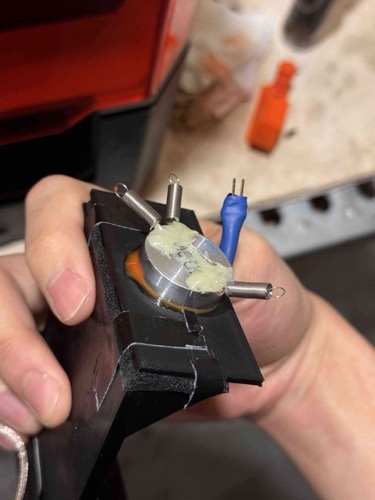
\includegraphics[width=0.3\textwidth,,valign=c]{photos/IMG_9604.jpg} & 
Now the surface transducer is permanently mounted to the housing plate.  \\ 
\hline

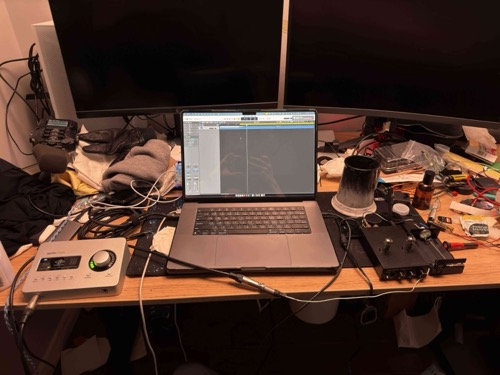
\includegraphics[width=0.3\textwidth,,valign=c]{photos/IMG_9605.jpg} & 
Final recording setup completed. \\ 
\hline



\end{longtable}



\newpage
\section{Recording setup}
I connected my iPhone to the amplifier, which drives the surface transducer via \textbf{Bluetooth}. The piezoelectric pickup, attached to the spring, was connected to my sound interface, the \textbf{Apollo Solo}, which in turn was connected to my laptop. I recorded the reverb effect using \textbf{Logic Pro}. Then, I played the test clip from my phone and started recording in Logic Pro.

Due to the piezo pickup being designed for guitar use, its sensitivity was insufficient for capturing vibrations from the spring. Therefore, I had to increase the gain for the piezo pickup to +52 dB on the sound interface (hardware gain) to capture any sound, which also amplified the noise. Subsequently, I have to use the \textbf{X-noise} plugin from Waves to mitigate these noises, otherwise we cannot compare the spectrum later on. Even though applying the noise reduction plugin resulting in reduced detail.


\begin{figure*}[h]
\center
	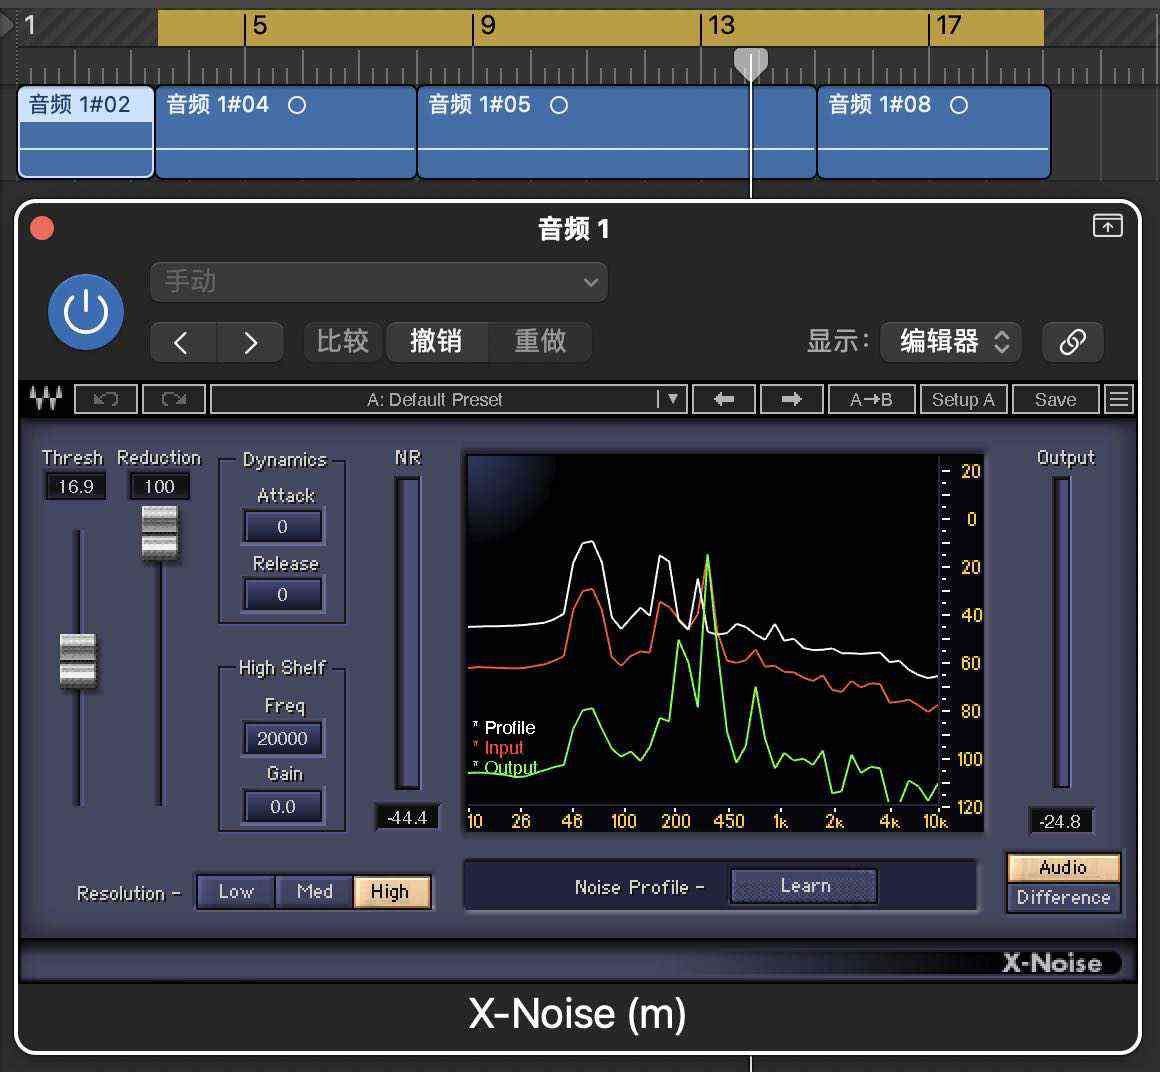
\includegraphics[width=0.5\linewidth]{photos/xnoise.jpg}
	\caption{Using plugin to cancel the noises}
\end{figure*}


\section{Future developments}

During my recording process, I found that when I turn the amplifier for the surface transducer too high, it would result in the spring touching itself (too much vibration on the spring), which will create some rather loud artifact and disrupt the actual signal. So, I had to lower the signal, which resulted in me needing to +52 dB on the sound interface in recording, which resulted in an extensive amount of noise. 

\begin{figure*}[h] 
	\center 
	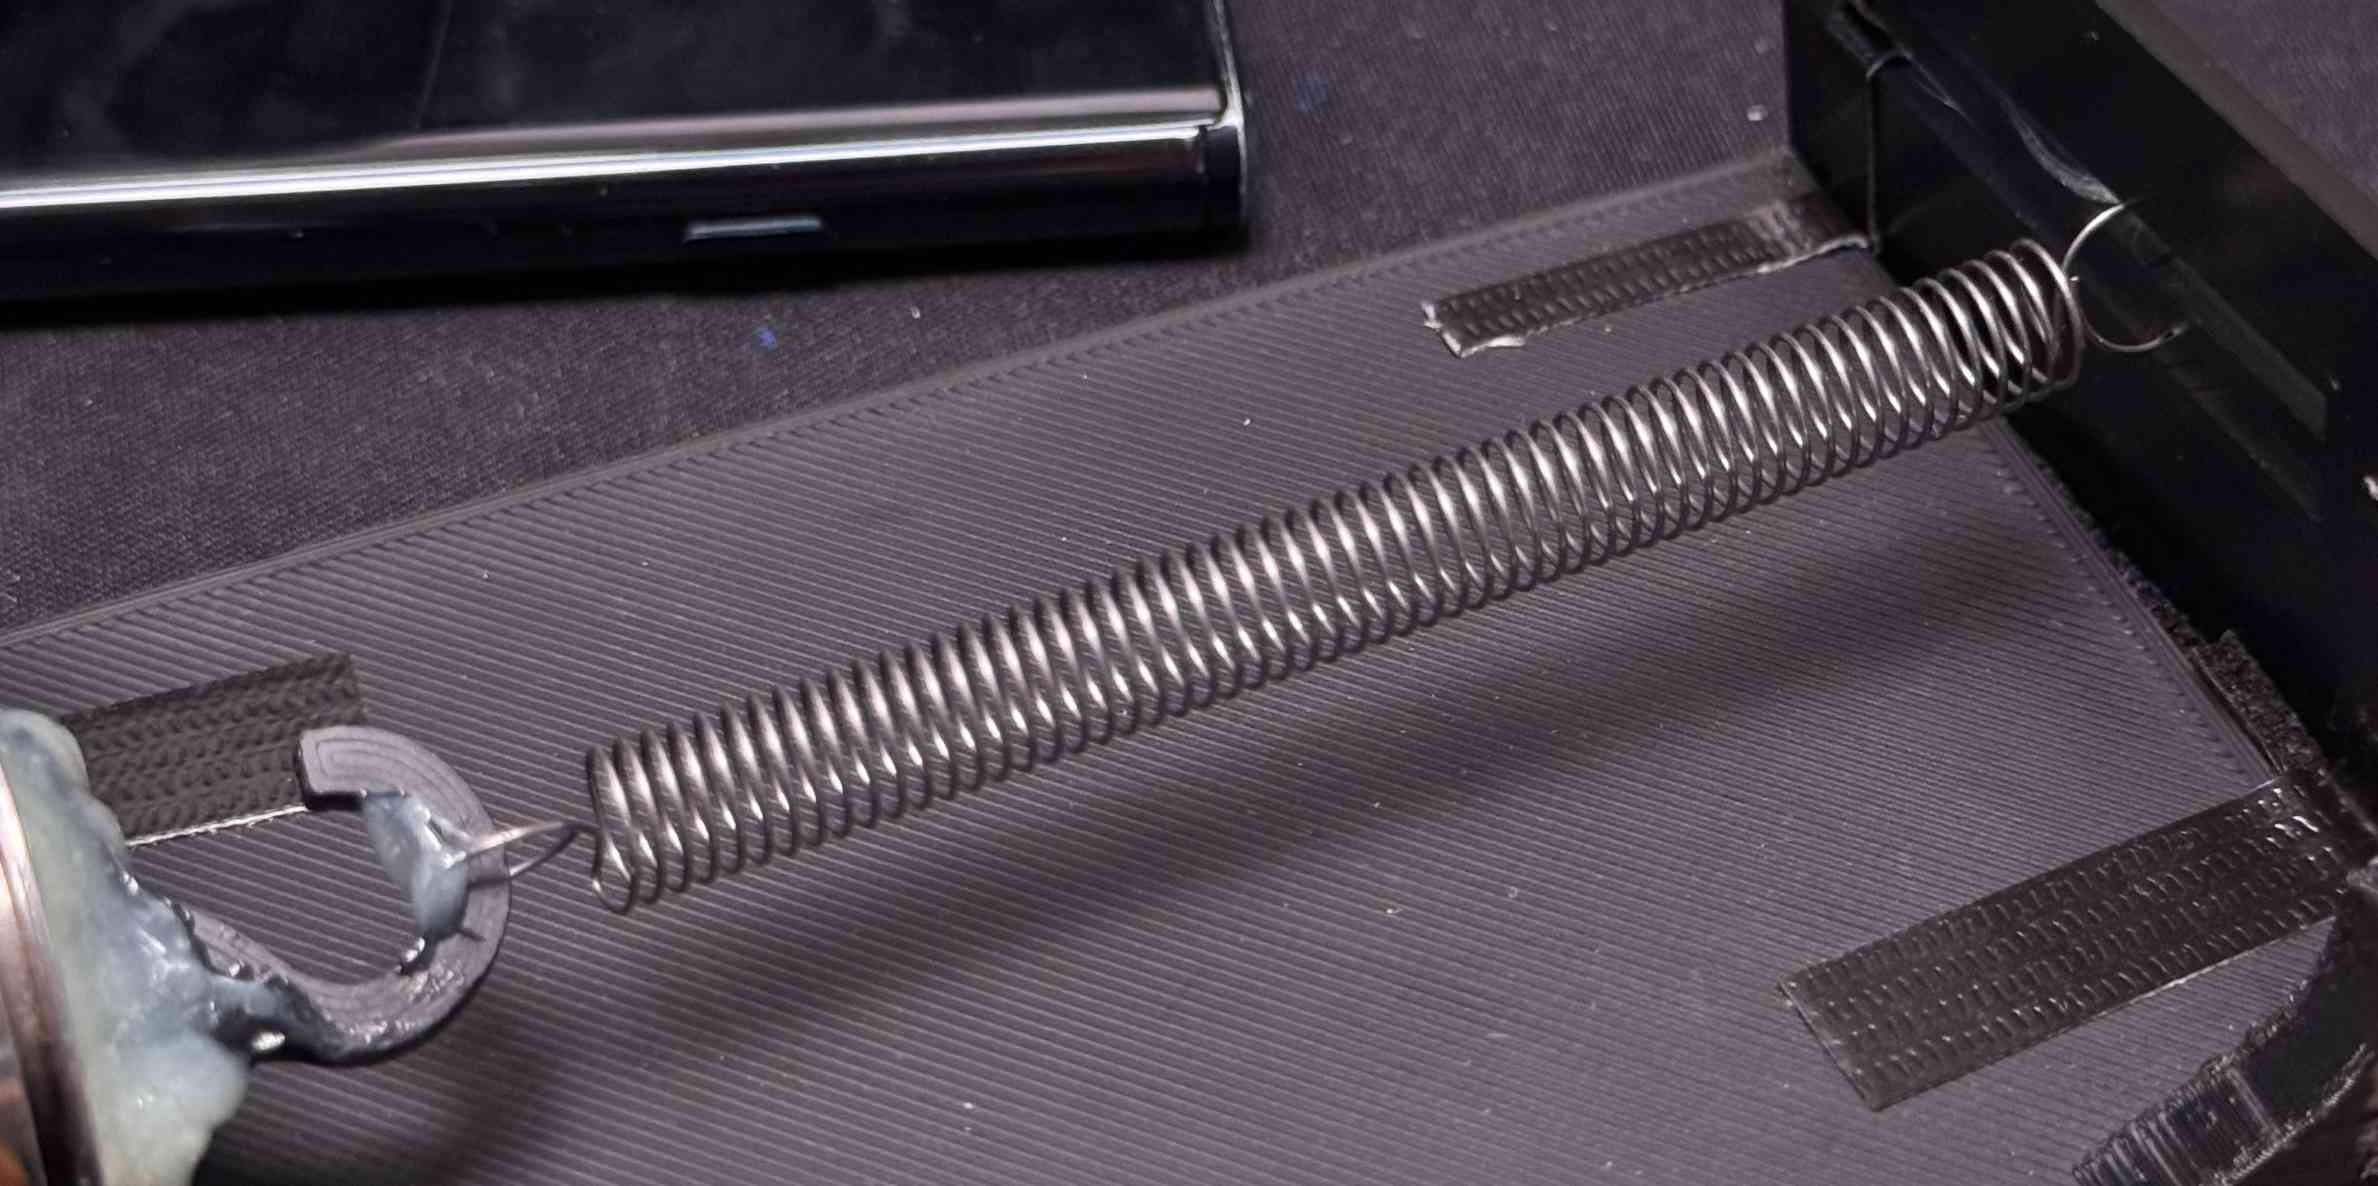
\includegraphics[width=0.5\linewidth]{photos/spring.jpg} 
	\caption{Spring used in my reverb tank} 
\end{figure*} 


I think this is mainly due to the fact that the spring I used has too many coil numbers, so it's very easy for the coils to touch each other when the amplitude is large. To mitigate this, I will have to find some extension spring that has the same diameter for the wire but way less coil number. However, the one I got is the only one left in the E3 mechanical store. So finding a suitable spring is quite hard and couldn't be completed in time for this project. 

Secondly, even though the spring is not that suitable, the piezo pickup is definitely not sensitive enough for usage to capture vibrations of the spring. To improve this, I will need to find some other piezo pickup systems that are not designed for under-saddle usage for guitars, rather for sticking on the surface of an instrument to capture sound, which should be more sensitive. Also, this couldn't be accomplished due to the time constraints of this project. 

Lastly, the use of foam tape with duct tape seems quite effective for stopping the vibration, but after sitting for a few days, it shows some level of deformation under the tension of the spring. So, some other mechanism not involving duct tape and foam tape is needed. I was originally thinking of use the spring to suspend the surface transducer somewhere, but the supporting structure for this seems not possible to be 3D printed. Also, to design and actually create such structure is also impossible to accomplished due to the time constraints of this project.

\begin{figure*}[h] 
	\center 
	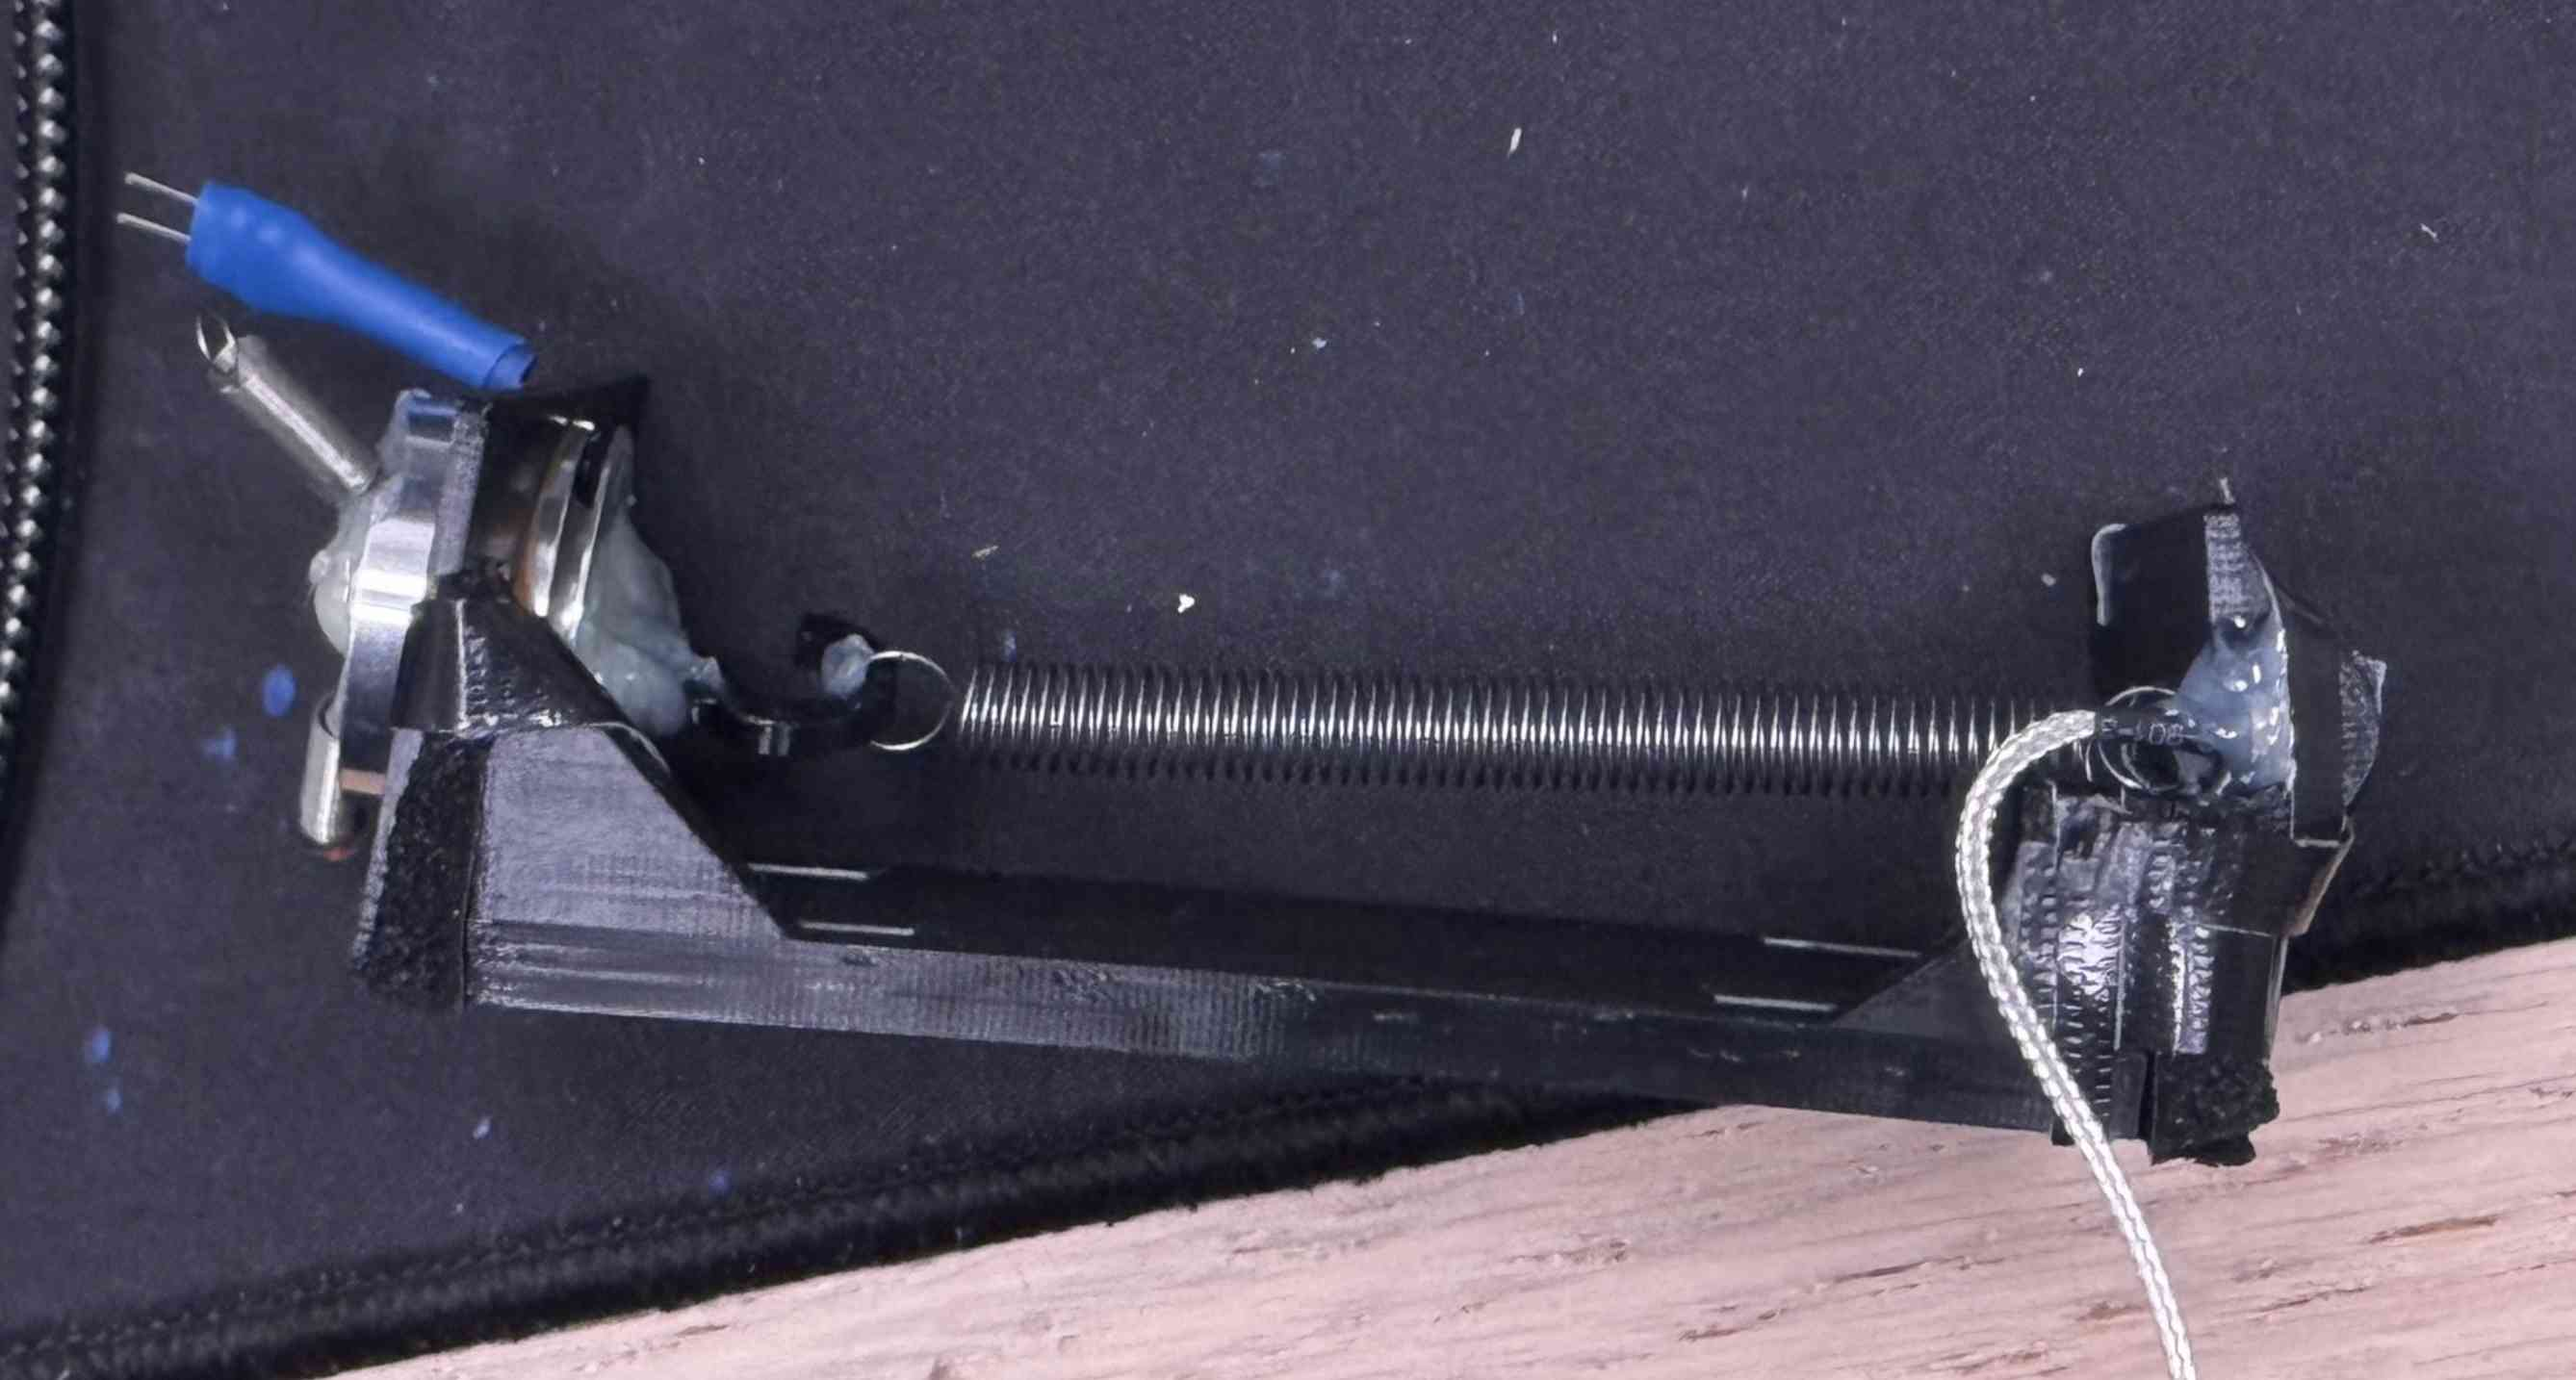
\includegraphics[width=0.5\linewidth]{photos/deformation.jpg} 
	\caption{Housing is no longer straight under the tension of the spring} 
\end{figure*} 


\end{document}
